\documentclass[11pt]{article}
\usepackage[utf8]{inputenc}	% Para caracteres en español
\usepackage{amsmath,amsthm,amsfonts,amssymb,amscd}
\usepackage{multirow,booktabs}
\usepackage[table]{xcolor}
\usepackage{fullpage}
\usepackage{lastpage}
\usepackage{enumitem}
\usepackage{fancyhdr}
\usepackage{mathrsfs}
\usepackage{wrapfig}
\usepackage{setspace}
\usepackage{hyperref}
\usepackage{calc}
\usepackage{multicol}
\usepackage{cancel}
\usepackage[retainorgcmds]{IEEEtrantools}
\usepackage[margin=3cm]{geometry}
\usepackage{amsmath}
\newlength{\tabcont}
\setlength{\parindent}{0.0in}
\setlength{\parskip}{0.05in}
\usepackage{empheq}
\usepackage{framed}
\usepackage[most]{tcolorbox}
\usepackage{xcolor}
\colorlet{shadecolor}{orange!15}
\parindent 0in
\parskip 12pt
\geometry{margin=1in, headsep=0.25in}
\theoremstyle{definition}
\usepackage{pdfpages}
\newtheorem{defn}{Definition}
\newtheorem{reg}{Rule}
\newtheorem{exer}{Exercise}
\newtheorem{note}{Note}
\usepackage{fancyhdr}\usepackage{xcolor}\usepackage{amsmath}\usepackage{amssymb}\pagestyle{fancy}\rhead{}
\newtheorem{theorem}{Theorem}[subsection]
\theoremstyle{definition}
\newtheorem{definition}[theorem]{Definiton}
\newtheorem{example}[theorem]{Example}
\newtheorem{corollary}[theorem]{Corollary}
\newtheorem{lemma}[theorem]{Lemma}
\title{Chapter 9 Review Notes}
\begin{document}
\thispagestyle{empty}
{\LARGE \bf CIV 102 Lecture Notes}\\
{\large Hei Shing Cheung}\\
Structures and Materials, Fall 2024 \hfill CIV102\\
\\
The up-to-date version of this document can be found at \url{https://github.com/HaysonC/skulenotes}\\

\begin{center}
\textit{"Structural Engineering is the art and science of designing and molding structures with economy and elegance so that they can safely resist the force that they are subjected''} \\ - Prof. \textsc{Evan Bentz, 2024}
\end{center}
\vspace{10pt}
\section{Force, Moment, and Geometry} 
    \paragraph{Moment for One Force} The moment due to only one force is:
    \begin{equation}
        \mu = \mathrm{moment} = \Vec{F}\times\Vec{d_\perp}
    \end{equation}
Where:
\begin{equation*}
\begin{split}
\Vec{d_\perp} = \text{The perpendicular displacement to the center of rotation}
\end{split}
\end{equation*}
\paragraph{Centroid} The centroid of a shape with multiple geometries is calculated by: 
\begin{equation}
\bar{y} = \frac{\sum_i A_i  y_i}{\sum_i A_i}
\end{equation}
\paragraph{Parallel axis Theorem} The moment of inertia is calculated by the following
\begin{equation}
    I = \sum_i I_{i} + \sum_i A_i d_i^2
\end{equation}
Where:
\begin{equation*}
\begin{split}
d_i = \text{The displacement of $\bar{y_i}$ to $\bar{y}$}
\end{split}
\end{equation*}
\paragraph{First Moment of Area (Q)} It is expressed as.
\begin{equation}
    Q = \sum_i A_i \cdot d_i
\end{equation}
\section{Truss}
\paragraph{Area} Design area against tension/compression by:
\begin{equation}
    A \geq \frac{2F}{\sigma_y}
\end{equation}
\paragraph{Moment of Intertia} Design MOI against Euler's bucking by:
\begin{equation}
    I \geq \frac{3FL^2}{\pi^2E}
\end{equation}
\paragraph{Radius of Gyration} Design radius of gyration against slenderness ratio by:
\begin{equation}
    r \geq \frac{L}{200}
\end{equation}
\section{Beam}
\paragraph{Navier's equation} 
\begin{equation}
    \sigma = \frac{My}{I}
\end{equation}

\paragraph{Curvature Equation}
\begin{equation}
    \phi = \frac{M}{EI}
\end{equation}

\paragraph{MAT 1} The change in slope between two points is given by the first moment area theorem:
\begin{equation}
    \Delta_{AB} = \theta_B - \theta_A = \int_A^B \phi(x) \, dx
\end{equation}

\paragraph{MAT 2} The deviation of point $A$ from the tangent drawn at point $B$ is given by the second moment area theorem:
\begin{equation}
    EIt_{A/B} = \int_B^A x M(x) \, dx = \bar{x}_{AB} \int_B^A M(x) \, dx
\end{equation}
\paragraph{Shear Stress} Given by Jourawski's equation:
\begin{equation}
    \tau = \frac{VQ}{Ib}
\end{equation}
\section{Virtual Work}
\paragraph{Work} In elastic deformation, for internal energy, we have
$$
W_\text{int} = V\frac{\sigma \epsilon}{2} = \frac{P\Delta}{2}
$$
In Hookes Law, for external energy, we have:
$$
W_\text{ext} = F\Delta r
$$
\paragraph{Change of length} For a change of length, we have 
\begin{equation}
\Delta = \frac{PL}{EA}
\end{equation}
\paragraph{Deflection} to calculate bean deflection, we sum the total virtual force multiplied by extension (worked done by victual forces, virtual work):
\begin{equation}
    F^\star \Delta_{\hat{r}} = \sum_{i}P^\star_i \Delta_i
\end{equation}
\section{Vibraion}
\subsection{Free Vibration}
Since for change of length, we have:
\begin{align}
    \Delta = \frac{PL}{EA} \nonumber 
    \intertext{This could be rewritten as: }
    P = \frac{EA}{L}\Delta \nonumber
    \intertext{For stiffness $k$, this could be molded as a simple harmonic motion with:}
    k = \frac{EA}{L}
\end{align}
\paragraph{For Truss} We can use the method of virtual load to determine $\Delta_0$. 
\paragraph{For Beam} We can use the method of MAT to determine $\Delta_0$.
\paragraph{Point Load} The natural frequency is: \begin{equation}
f_n = \frac{15.76}{\sqrt{\Delta_0}}
\end{equation}
\paragraph{Uniform Load} The natural frequency is 
\begin{equation}
f_n = \frac{17.76}{\sqrt{\Delta_0}}
\end{equation}
\paragraph{Dynamic Amplification Factor} Denoted as DAF, for forced vibration at a frequency $f$, DAF is computed as:
\begin{equation}
    \text{DAF} = \frac{1}{\sqrt{(1-(\frac{f}{f_n})^2)^2+ (2\beta \frac{f}{f_n})^2}}
\end{equation}
\paragraph{Amplification} Members would be subject to loads $\text{DAF} \times P$ when the load is vibrating. 
\section{Shear and Local Buckling}
\begin{table}[ht]
\centering
\caption{Summary of plate buckling failure modes}
\begin{tabular}{|l|l|l|}
\hline
\textbf{Failure Mode}                                           & \textbf{Failure Condition}                                                                                      & \textbf{Equation}                          \\ \hline
Buckling of the compressive flange                              & $\sigma = \dfrac{4 \pi^2 E}{12 (1 - \mu^2)} \left( \dfrac{t}{b} \right)^2$                                      & $\sigma = \dfrac{M y}{I}$                                  \\
between the webs                                                &                                                                                                                &                                                           \\ \hline
Buckling of the tips of the                                     & $\sigma = \dfrac{0.425 \pi^2 E }{12 (1 - \mu^2)} \left( \dfrac{t}{b} \right)^2$                                & $\sigma = \dfrac{M y}{I}$                                  \\
compressive flange                                              &                                                                                                                &                                                           \\ \hline
Buckling of the webs due to the                                 & $\sigma = \dfrac{6 \pi^2 E}{12 (1 - \mu^2)} \left( \dfrac{t}{b} \right)^2$                                      & $\sigma = \dfrac{M y}{I}$                                  \\
flexural stresses                                               &                                                                                                                &                                                           \\ \hline
Shear buckling of the webs                                      & $\tau = \dfrac{5 \pi^2 E}{12 (1 - \mu^2)} \left( \left( \dfrac{t}{h} \right)^2 + \left( \dfrac{t}{a} \right)^2 \right)$ & $\tau = \dfrac{V Q}{I b}$                                  \\ \hline
\end{tabular}
\end{table}
\section{Concrete}
\subsection{Material Properties}
\paragraph{Tensile Strength} The compressive strength and the tensile strength of concrete is related as follows:
\begin{equation}
    f'_t = 0.33\sqrt{f'_c}
\end{equation}
\paragraph{Young's Modulus} The compressive strength and the Young's modulus of concrete is related as follows:
\begin{equation}
    E_c = 4730\sqrt{f'_c}
\end{equation}
\begin{shaded}
\textit{Typical Values}:\\
Steel's Young's modulus is usually $E_s = 200,000$ MPa and the yield strength is $f_y = 400$ MPa.
\end{shaded}


The modular ratio $n$ is given as:
\begin{equation}
    n = \frac{E_s}{E_c}
\end{equation}

The quantity of longitudinal reinforcement $\rho$ is given as:
\begin{equation}
    \rho = \frac{A_s}{bd}
\end{equation}
where:
\begin{equation*}
\begin{split}
    A_s = \text{The area of the steel reinforcements.}\\
    b = \text{The width of the cross-sectional region of interest.}\\
    d = \text{The distance from the edge of the region of interest to the opposing reinforcements.}
\end{split}
\end{equation*}  

\paragraph{$k$, Scaling Factor} of extreme compression fiber to the neutral axis is given as:
\begin{equation}
    k = \sqrt{(n\rho)^2 + 2n\rho} - n\rho
\end{equation}
\paragraph{$j$, Scaling factor } of the flexural lever is given as:
\begin{equation}
    j = 1 - \frac{1}{3}k
\end{equation}
\begin{shaded}
    \textit{Typical Values:}\\  The scaler factors are usually $k = \frac{3}{8}$ and $j = \frac{7}{8}$.
\end{shaded}

\subsection{Flexural Stress Analysis}
\paragraph{In Reinforcement} The stress is given by:
\begin{equation}
    f_s = \frac{M}{A_s j d}
\end{equation}
\paragraph{In Concrete} The stress is given by:
\begin{equation}
    f_c = \frac{k}{1-k} \cdot \frac{M}{n A_s j d}
\end{equation}

\subsection{Shear Stress Analysis}
\paragraph{Maximum Shear Stress in Cracked Concrete}
The maximum shear stress $v$ in a cracked concrete member's web is given by:
\begin{equation}
    v = \frac{V}{b_w j d}
\end{equation}
where $b_w$ is the effective web width.

\paragraph{Buckling Shear Stress}
The shear stress $v_{\text{max}}$ that causes buckling from diagonal compression is:
\begin{equation}
    v_{\text{max}} = 0.25 f'_c
\end{equation}
\paragraph{Steps for checking Shear Stress} Steps by step, if the shear strength does not pass the conditions below:
\begin{itemize}
    \item \textbf{Concrete Crushing Limit} Concrete will crush when:
    \begin{equation}
        V \geq \min(V_r, V_{\text{max}})
    \end{equation}
    where:
    \begin{equation}
    V_{\text{max}} = 0.25 f'_c b_w j d
    \end{equation}
    \item \textbf{Shear Strength of the Member}
    The shear strength $V_r$ of the member is:
    \begin{equation}
        V_r = V_c + V_s
    \end{equation}
    \item \textbf{Safety Factor for Design}
    For design purposes, select $V_r$ such that:
    \begin{equation}
        V_r = 0.5 V_c + 0.5 V_s \leq 0.5 V_{\text{max}}
    \end{equation}
\end{itemize}
Then we pass on another case  below if it involves $V_r$
\begin{itemize}
    \item \textbf{Without Reinforcement} If no shear reinforcement is present, the shear strength $V_c$ of the concrete is:
    \begin{equation}
        V_c = 230 \sqrt{f'_c} + 0.9 d b_w j d
    \end{equation}
    \item \textbf{With Minimum Reinforcement} When using shear reinforcement (stirrups), the shear strength $V_c$ of the concrete is:
    \begin{equation}
        V_c = 0.18 \sqrt{f'_c} b_w j d
    \end{equation}
    This equation is valid if:
    \begin{align}
        \frac{A_v f_y}{b_w s} 
 & \geq 0.06 \sqrt{f'_c}\\
        \Leftrightarrow s & \leq \frac{A_v f_y}{0.06 \cdot b_w \cdot \sqrt{f'_c}} \nonumber
    \end{align}
    where:
    \begin{equation*}
    \begin{split}
    A_v= \text{The effective area of stirrups; and}\\
    s = \text{Spacing between stirrups}
    \end{split}
    \end{equation*}
    \item \textbf{With Additional Reinforcement} If shear reinforcement is used, the maximum shear force $V_s$ carried is:
    \begin{equation}
        V_s = \frac{A_v f_y j d}{s} \cot(35^\circ)
    \end{equation}
\end{itemize}

\paragraph{Design Suggestions for Safety}
If a design is unsafe, consider the following:
\begin{itemize}
    \item If $V \geq 0.5 V_{\text{max}}$, resize the cross-section.
    \item If $V \geq 0.5 V_c$, add reinforcements.
    \item If $V \geq 0.5 V_c + 0.5 V_s$, adjust the spacing $s$:
    \begin{equation}
    s = \frac{0.5 A_v f_y j d \cot(35^\circ)}{V - 0.5 \times 0.18 \sqrt{f'_c} b_w j d}
    \end{equation}
\end{itemize}
\appendix
\newpage
\rhead{CIV Formula Booklet}
\lhead{\leftmark}
\pagenumbering{alph}

\section{Common Op-Amp Circuits} \label{app:OpAmpCircuits}
\begin{figure}[h!]
    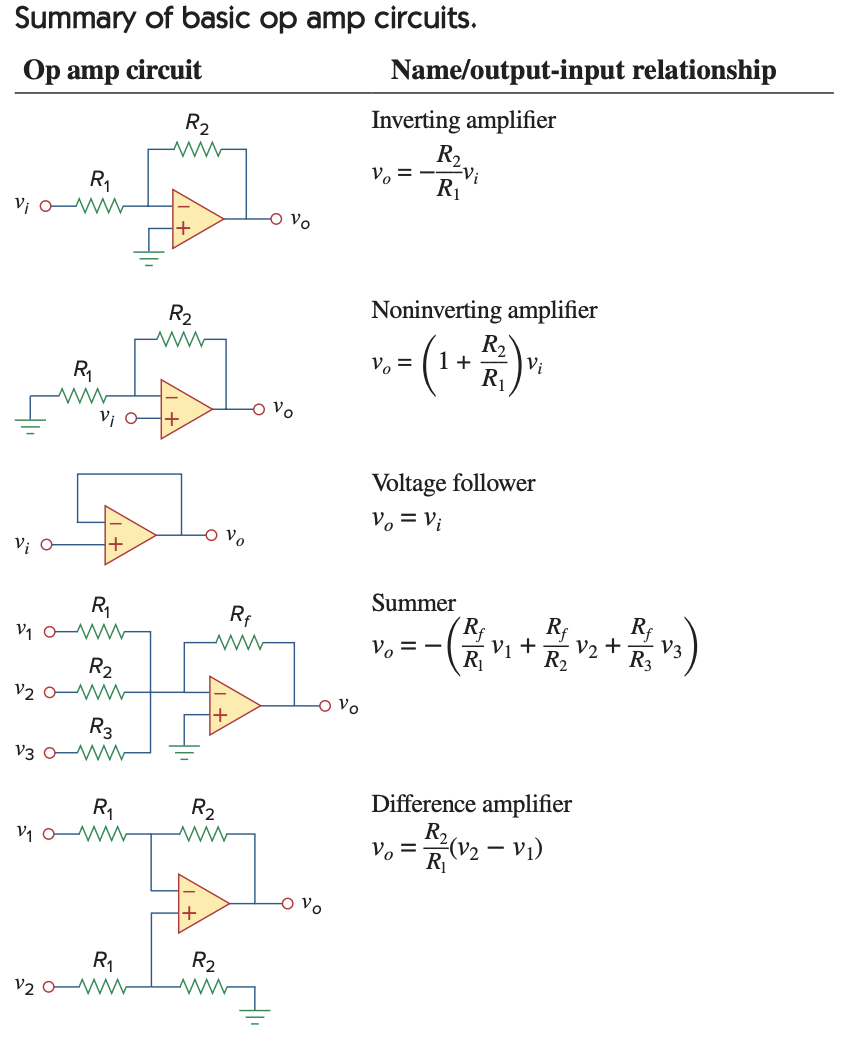
\includegraphics[width=0.9\linewidth]{AppendixItems/OpAmps.png}
    \centering
    \caption{Common Op-Amp Circuits}
\end{figure}
\end{document}